\begin{fullwidth}
\chapter[MTH1’S RESULTS]{Mth1’s results}
\label{chap:res1}
\end{fullwidth}

\marginnote{\adforn{42} \Chapref{chap:mth1} \hfill \Chapref{chap:sota2} \adforn{43}}

\paragraph{Synopsis}
This chapter presents the results we obtained with METHOD1. We start with … §\ref{sec:res1:sec1}, and we continue with … §\ref{sec:res1:sec2}.

% =======================================================

\section{sec1}
\label{sec:res1:sec1}
This section compares …

% -------------------------------------------------------

\subsection{Figures examples}

\paragraph{Single figure} Figure \ref{fig:res1:fig1} shows … \blindtext

\begin{figure}
  \centering
  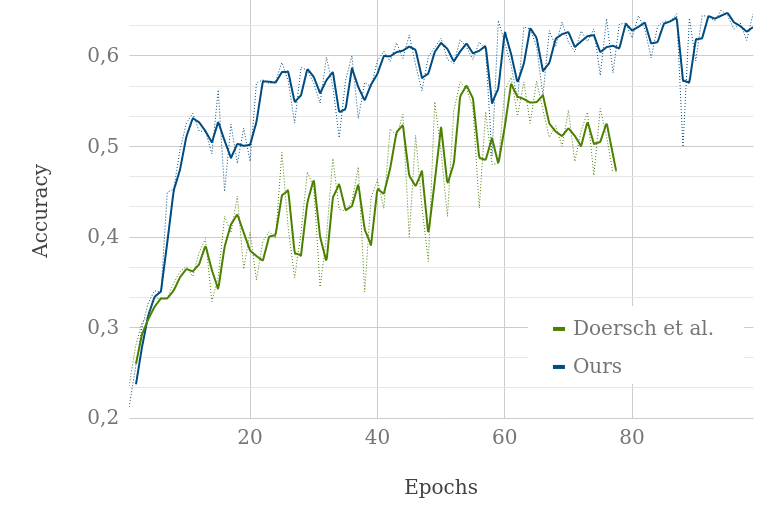
\includegraphics[width=\linewidth]{30-part1/img/resultsicip.png}
  \caption[Validation accuracy --- Comparison of our architecture and Doersch et al.’s]{Validation accuracy scores --- Comparison of our architecture and Doersch et al.’s.}
  \label{fig:res1:fig1}
\end{figure}

\paragraph{Double figure} Figure \ref{fig:res1:fig3} shows … \blindtext

\begin{figure}
    \centering
    \subfloat[\label{fig:dz:09_sol}]{\qquad}
    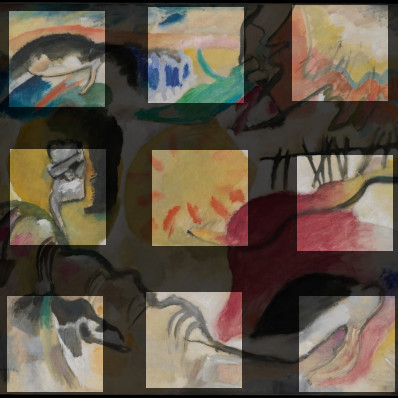
\includegraphics[width=0.4\linewidth]{30-part1/img/09_sol.jpg}\hfill
    \subfloat[\label{fig:dz:09_rea}]{\qquad}
    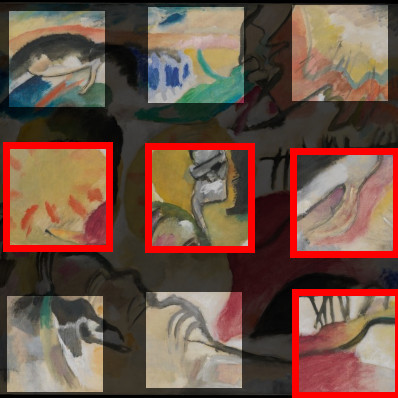
\includegraphics[width=0.4\linewidth]{30-part1/img/09_res.jpg}
    \caption[An erroneous reassembly with unknown center]{Example of a wrong reassembly with unknown center. The red outline shows the fragments that are misplaced  --- Fig. \protect\subref{fig:dz:09_sol} shows the expected outcome, and Fig. \protect\subref{fig:dz:09_rea} the predicted result.}
    \label{fig:res1:fig3}
\end{figure}

\begin{marginfigure}[25em]
    \centering
    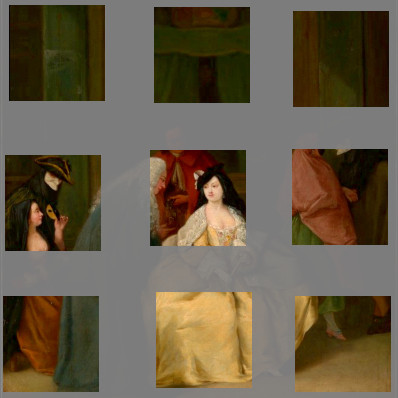
\includegraphics[width=\linewidth]{30-part1/img/05.jpg}
    \caption[A reassembly]{A typical reassembly.}
    \label{fig:res1:fig2}
\end{marginfigure}

\paragraph{Margin figure} Figure \ref{fig:res1:fig2} illustrates … \blindtext

\paragraph{Full width figure} Figure \ref{fig:res1:fig4} shows … \blindtext

\begin{figure*}
    \centering
    \subfloat[\label{fig:dzr:20a}]{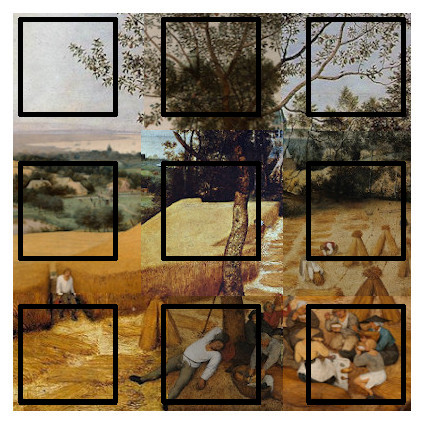
\includegraphics[width=0.23\textwidth]{30-part1/img/bruegel_sol.jpg}}\hfill
    \subfloat[\label{fig:dzr:20b}]{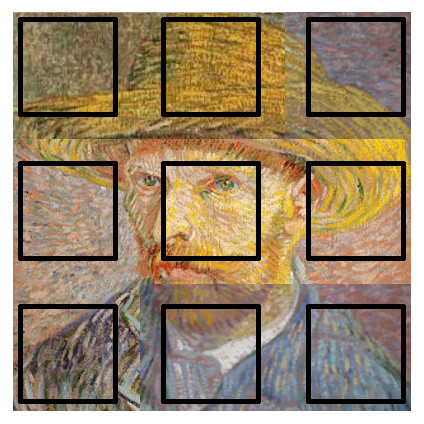
\includegraphics[width=0.23\textwidth]{30-part1/img/vg_sol.jpg}}\hfill
    \subfloat[\label{fig:dzr:20c}]{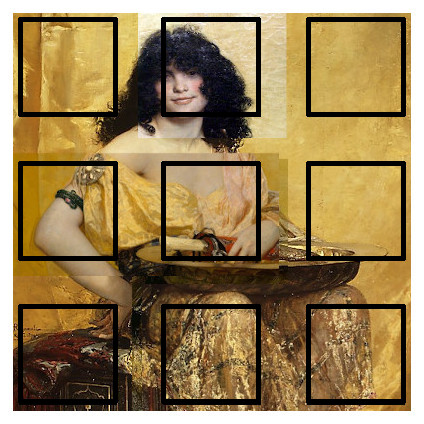
\includegraphics[width=0.23\textwidth]{30-part1/img/salom_sol.jpg}}\hfill
    \subfloat[\label{fig:dzr:20d}]{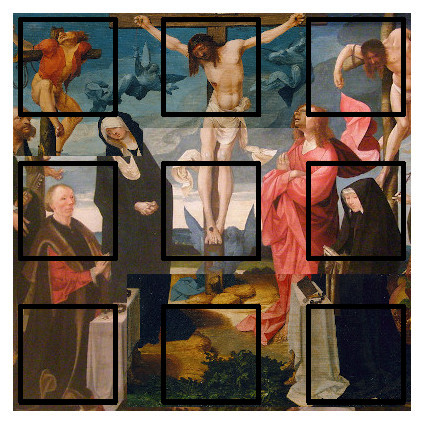
\includegraphics[width=0.23\textwidth]{30-part1/img/corn_sol.jpg}}

    \subfloat{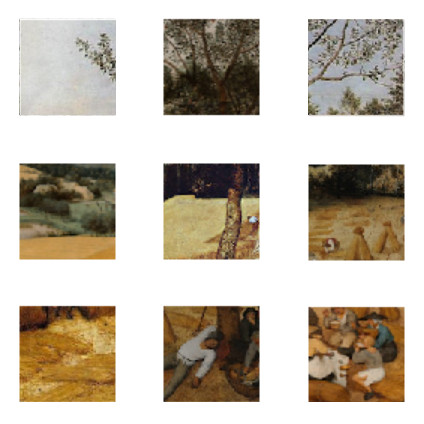
\includegraphics[width=0.23\textwidth]{30-part1/img/bruegel_res.jpg}}\hfill
    \subfloat{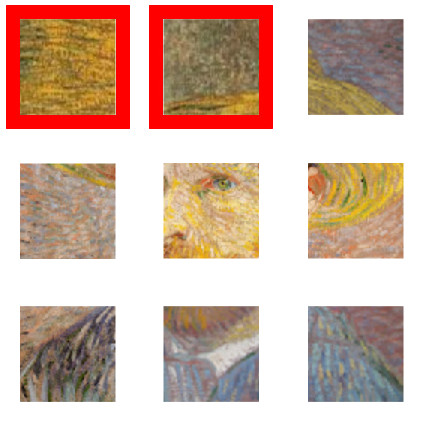
\includegraphics[width=0.23\textwidth]{30-part1/img/vg_res.jpg}}\hfill
    \subfloat{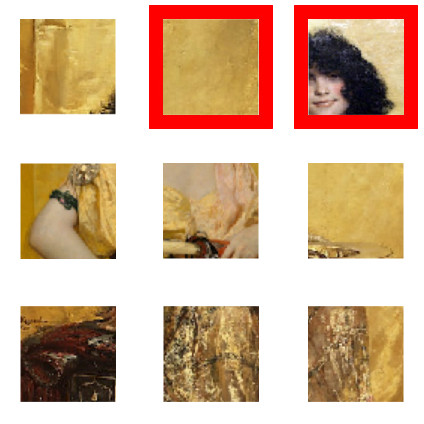
\includegraphics[width=0.23\textwidth]{30-part1/img/salom_res.jpg}}\hfill
    \subfloat{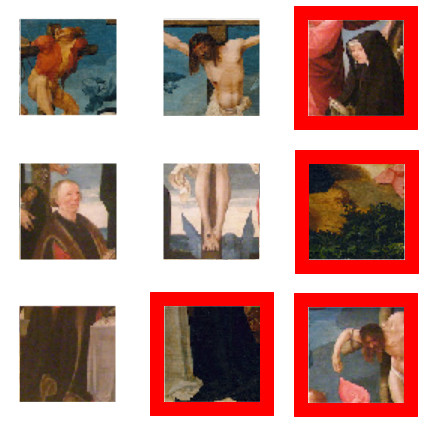
\includegraphics[width=0.23\textwidth]{30-part1/img/corn_res.jpg}}
\vspace{2em}
    \caption[Some reassemblies from patchwork images]{Reassemblies from patchwork images. The first row shows the patchwork images from which the fragments were extracted. The second row displays the reassemblies for the patchwork fragments. The third row contains the reassemblies of the MET image (without patchwork). The red outline shows the fragments that are misplaced. }
    \label{fig:res1:fig4}
\end{figure*}


% -------------------------------------------------------

\subsection{Tables examples}

Table \ref{tab:res1:tab1} compares … \blindtext

\begin{table}
    \centering
    \begin{tabular}{rrr}
        \toprule
        A & B & C \\
        \midrule
        - & - & - \\
        \bottomrule \\                           % don't forget \\
    \end{tabular}
    \caption[Validation accuracy --- Comparison between the setups]{Validation accuracy scores --- Comparison between the setups.}
    \label{tab:res1:tab1}
\end{table}

Table \ref{tab:res1:tab2} shows … \blindtext

\begin{table*}
  \centering
  \begin{tabular}{lrrrrr}
    \toprule
     &
    \multicolumn{2}{c}{Best attempt} &
    \multicolumn{2}{c}{Worst attempt} & \\
    \cmidrule(r){2-3}
    \cmidrule(r){4-5}
    \shortstack{Number \\ of attempt} & 
    \shortstack{Fragment-\\wise (\%)} & \shortstack{Puzzle-\\wise (\%)} &
    \shortstack{Fragment-\\wise (\%)} & \shortstack{Puzzle-\\wise (\%)} & \shortstack{Reassemblies\\done in 24h}\\
    \midrule
    - & - & - & - & - & - \\
    \bottomrule \\                              % don't forget \\
  \end{tabular}
  \caption[Reassembly --- Comparison of the order of fragments]{Reassembly scores --- Impact of the order of fragments.}
  \label{tab:res1:tab2}
\end{table*}

% =======================================================

\section{sec2}
\label{sec:res1:sec2}
This section …